\thispagestyle{timhieukhoahocnone}
\pagestyle{timhieukhoahoc}
\everymath{\color{timhieukhoahoc}}
\blfootnote{$^1$\text{\color{timhieukhoahoc}Hà Nội.}}
\graphicspath{{../timhieukhoahoc/pic2/}}
\begingroup
\AddToShipoutPicture*{\put(0,616){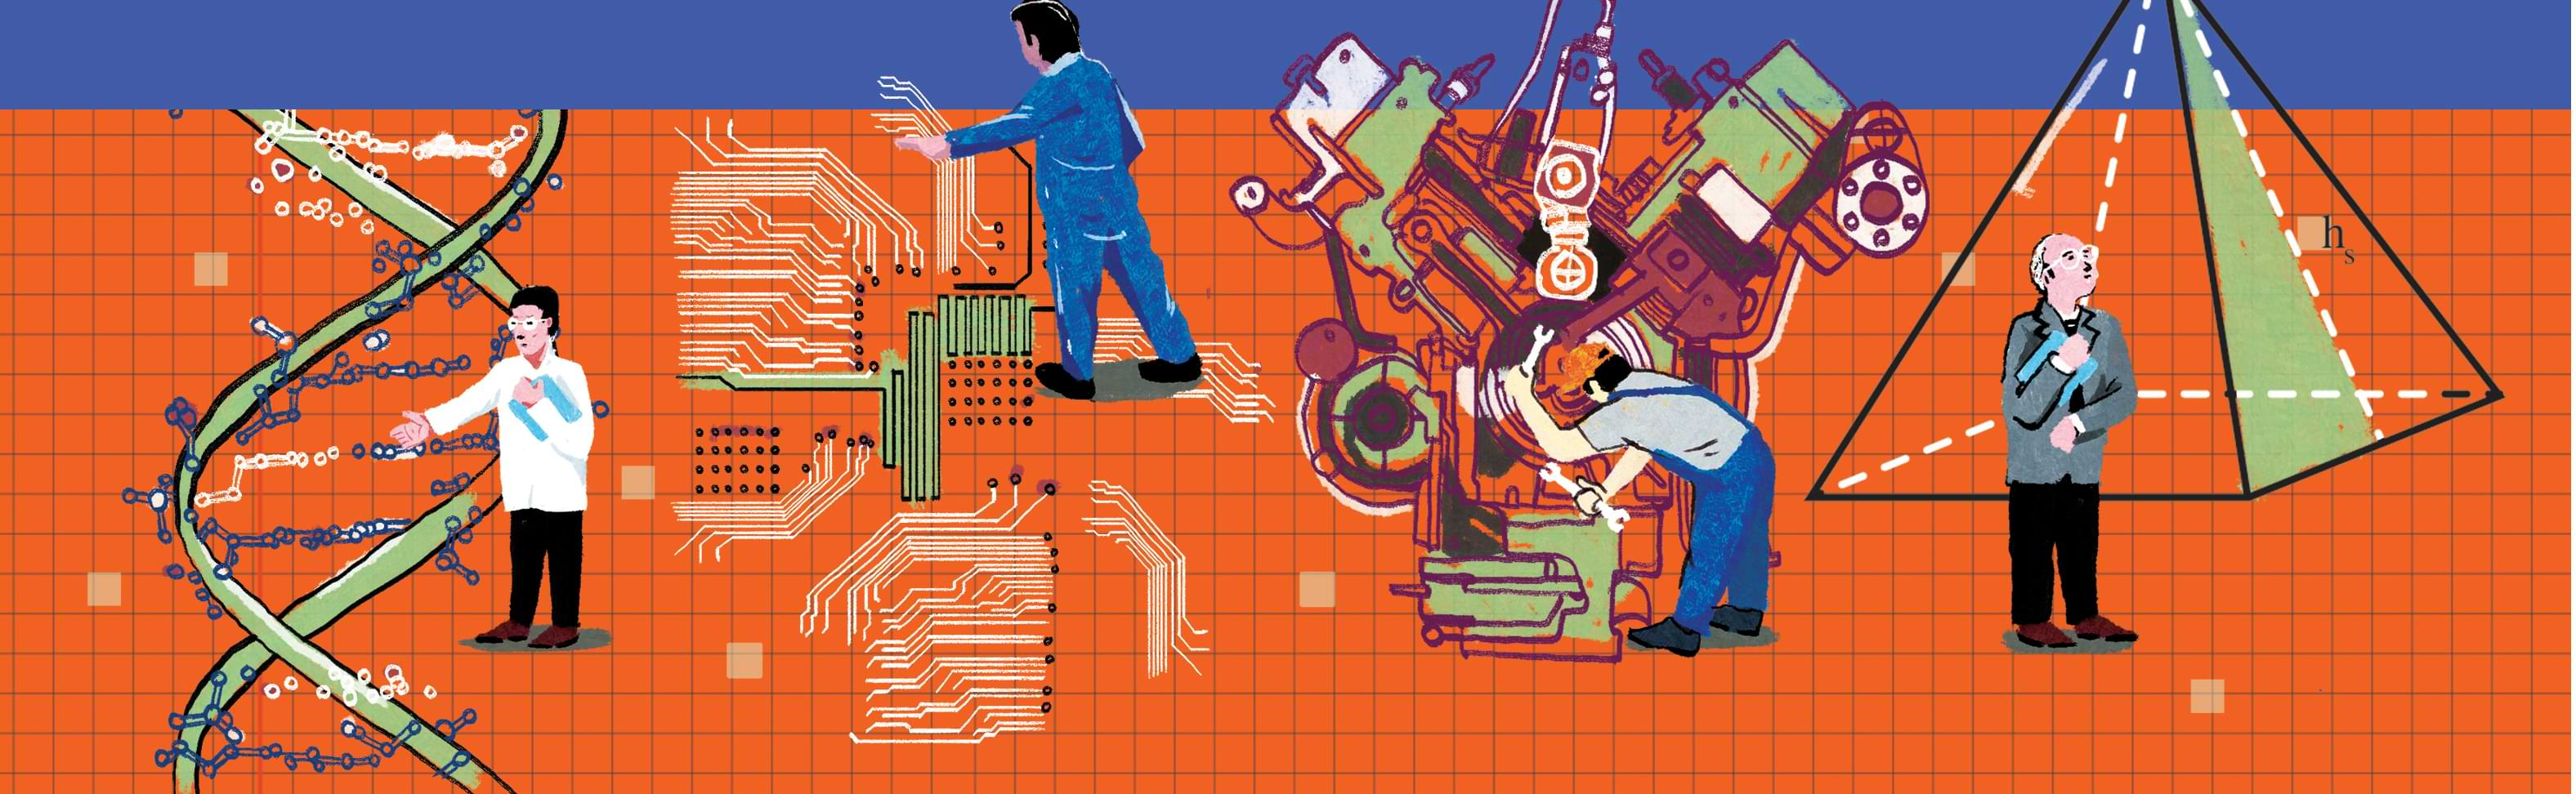
\includegraphics[width=19.3cm]{../bannertimhieu}}}
\AddToShipoutPicture*{\put(112,525){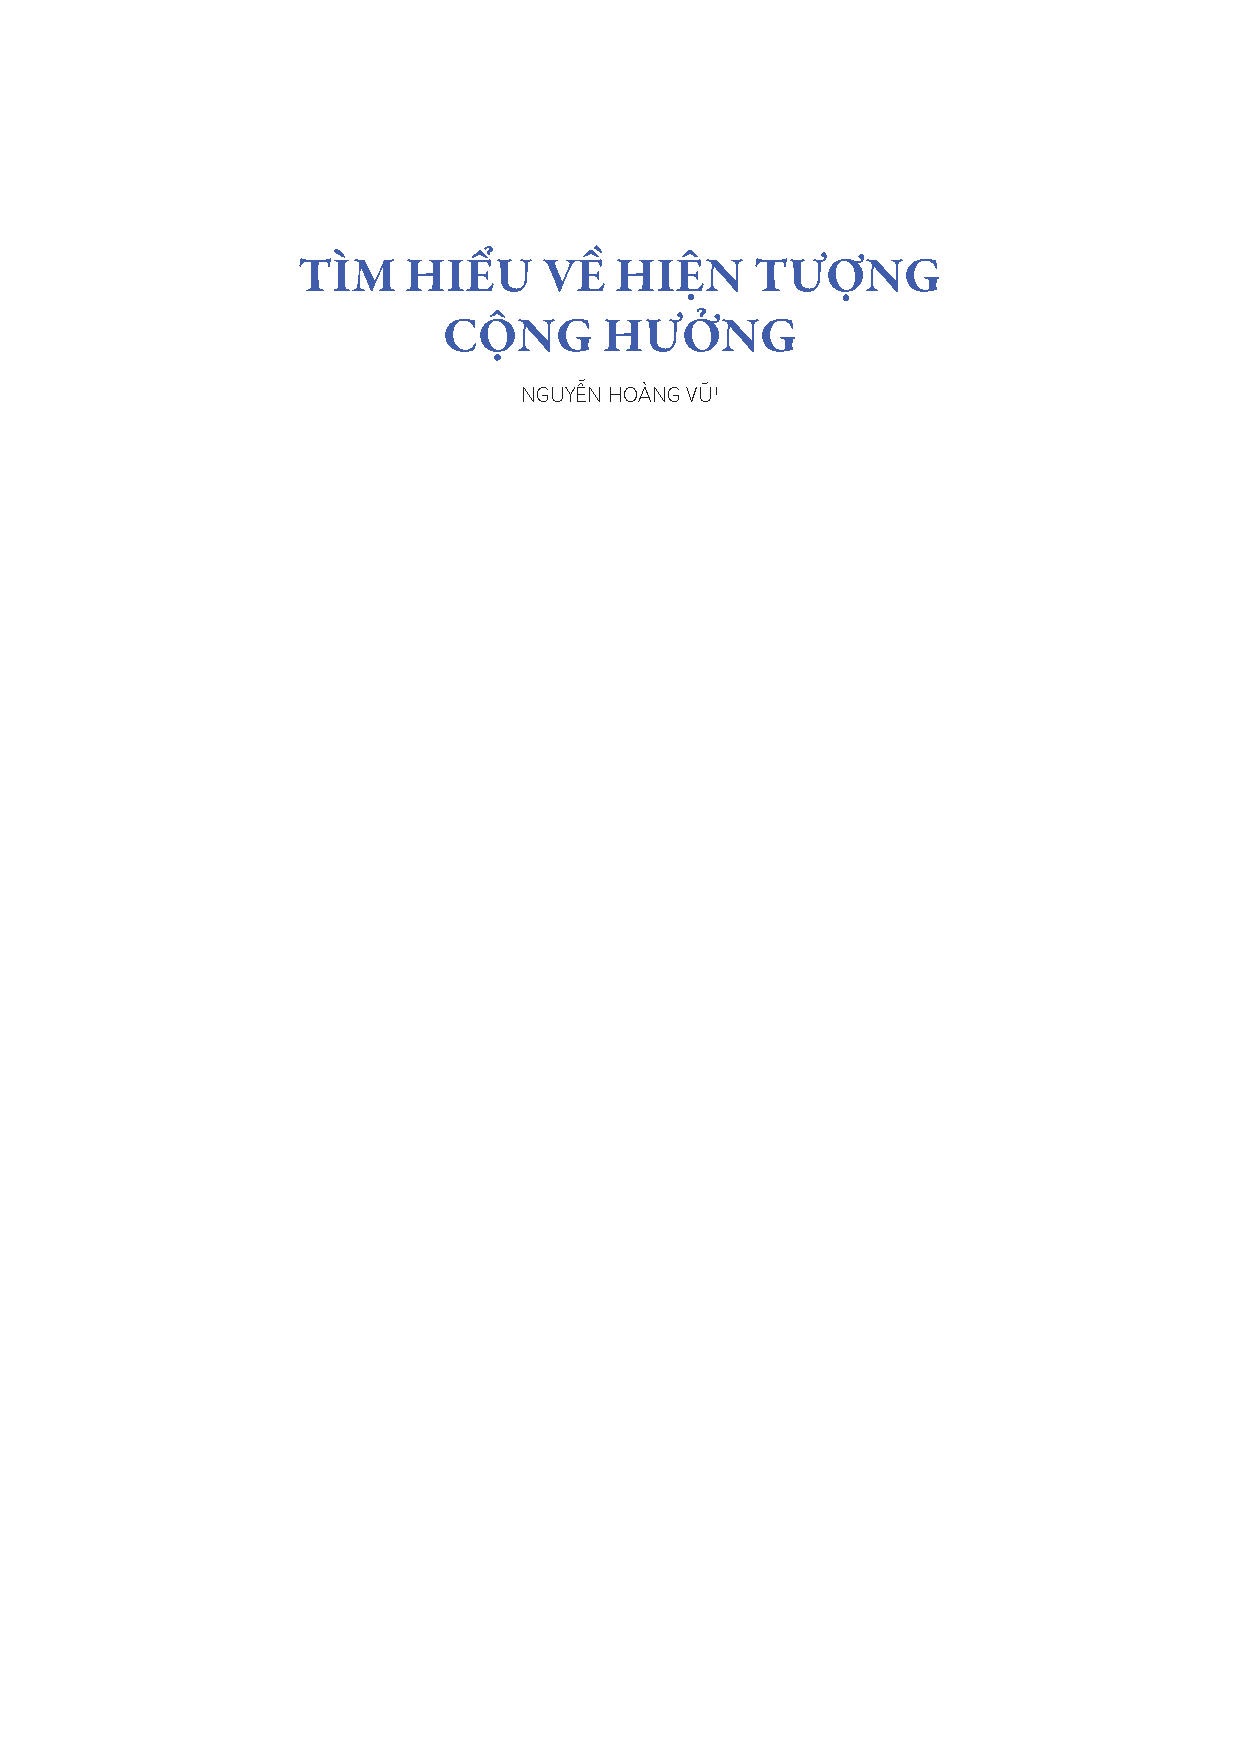
\includegraphics[scale=1]{../tieude.pdf}}}
\centering
\endgroup
\vspace*{178pt}

\begin{multicols}{2}
	Hiện tượng cộng hưởng là một nội dung kiến thức quan trọng trong chương trình vật lý lớp $12$. Nó xảy ra khi tác động từ bên ngoài có một tần số phù hợp làm biên độ của dao động bị tăng vọt. Trong bài viết này, chúng ta hãy cùng tìm hiểu về quá trình phát hiện của hiện tượng cộng hưởng cũng như một số ứng dụng thú vị của nó.
	\vskip 0.1cm
	$\pmb{1.}$ \textbf{\color{timhieukhoahoc}Mô hình cho thủy triều và bài toán dao động cưỡng bức}
	\vskip 0.1cm
	Hiện tượng cộng hưởng xuất hiện lần đầu tiên trong các tài liệu khoa học khi Galileo tiến hành giải thích về hiện tượng mang tính chu kỳ của thủy triều dựa trên các quan sát về dao động. Ông nhận thấy rằng một tác động yếu có thể làm tăng mạnh biên độ của một dao động nếu tác động này có một tần số phù hợp. Một ví dụ mà Galileo đưa ra là việc một quả chuông sau khi được một người tiến hành rung thì dây thừng của nó có thể nhấc bổng tận $6$ người lên. Sự tăng biên độ nhờ các tác động mang tính chu kỳ cũng có thể thấy được ở con lắc đơn trong đồng hồ hay các nhạc cụ dây.
	\vskip 0.1cm
	Galileo đưa ra một nhận định đúng đắn rằng mỗi một hệ dao động có một tần số dao động tự nhiên (dao động tự do). Tuy nhiên, ông lại cho rằng nó chỉ có thể có thể dao động với tần số này mà thôi (nhận định này không đúng). Sai lầm trên là một trong những nguyên nhân khiến Galileo kết luận rằng thủy triều được gây ra bởi chuyển động của Trái đất trong khi thực tế thì Mặt trăng có vai trò quan trọng liên quan đến chu kỳ của hiện tượng này.
	\vskip 0.1cm
	Phải đến thế kỷ $18$, tính chu kỳ của thủy triều lại được tiếp tục nghiên cứu bởi Euler. Ông đã tiến hành giải phương trình dao động với ngoại lực cũng là một hàm có chu kỳ. Bằng các công cụ giải tích, Euler đã tìm ra rằng nghiệm của trường hợp này là tổng của hai dao động điều hòa với hai tần số khác nhau. Tần số thức nhất phụ thuộc vào các tham số cấu tạo của hệ dao động và tần số thứ hai là tần số của ngoại lực. Euler giải được nghiệm đúng cho trường hợp hai tần số này bằng nhau và công thức nghiệm của ông cũng cho thấy sự tăng biên độ tuyến tính theo thời gian (tức khi cộng hưởng xảy ra). Tuy vậy, Euler không tiếp tục đi sâu vào phương diện vật lý của vấn đề này, ngoài việc nhắc đến sự liên hệ giữa nó và thủy triều. Trong các công trình sau này về cơ học, Euler cũng không quay lại bài toán trên, có thể là do ông chỉ xem nó như một câu hỏi toán học thú vị mà thôi.
	\vskip 0.1cm
	Đến thế kỷ $19$, Thomas Young, sau khi tiến hành thí nghiệm chứng minh bản chất sóng của ánh sáng năm $1802$, cũng bắt đầu nghiên cứu về mô hình của thủy triều. Ông tiến hành giải phương trình dao động dưới tác dụng của ngoại lực có chu kỳ giống như Euler nhưng thêm vào thành phần biểu diễn lực cản. Đồng thời, Young cũng đưa ra thuật ngữ dao động cưỡng bức để gọi tên trường hợp dao động này. Tuy nhiên, ông cũng vẫn chủ yếu tập trung vào giải thích tính chu kỳ của thủy triều mà không tiến hành mở rộng sang các ứng dụng cơ học khác. Khi các mô hình mới trong không gian $3$ chiều được đưa ra cho thủy triều thì mô hình dao động cưỡng bức của con lắc không còn được sử dụng nữa và nghiên cứu này của Young cũng không được chú ý đến. Đột phá thật sự chỉ xảy ra vài thập kỷ sau với các nghiên cứu của Helmholtz về sự cộng hưởng của sóng âm.
	\vskip 0.1cm
	$\pmb{2.}$ \textbf{\color{timhieukhoahoc}Helmholtz và sự cộng hưởng của sóng âm}
	\begin{figure}[H]
		\centering
		\vspace*{-5pt}
		\captionsetup{labelformat= empty, justification=centering}
		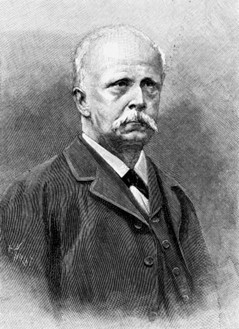
\includegraphics[width=1\linewidth]{1}
		\caption{\small\textit{\color{timhieukhoahoc}Hermann von Helmholtz ($1821 - 1894$).}}
		\vspace*{-10pt}
	\end{figure}
	Hermann von Helmholtz, sinh năm $1821$ tại Postdam, nay thuộc Đức, là con trai duy nhất của một giáo viên. Ông muốn học vật lý nhưng do hoàn cảnh tài chính nên theo học quân y bằng học bổng chính phủ. Trong thời gian làm bác sĩ phẫu thuật cho quân đội, Helmholtz vẫn có những đóng góp quan trọng trong vật lý, đặc biệt là sự thiết lập định luật bảo toàn năng lượng. Từ năm $1849$, ông giữ vị trí giáo sư ngành sinh lý học ở nhiều đại học khác nhau cho đến khi trở thành giáo sư vật lý tại đại học Humboldt, Berlin năm $1871$.
	\vskip 0.1cm
	Helmholtz bắt đầu các nghiên cứu về âm thanh vào năm $1856$, dựa trên các ý tưởng toán học của Fourier. Trước đó, khi giải bài toán về phương trình truyền nhiệt, Fourier đã đưa ra phương pháp biểu diễn một hàm số tuần hoàn dưới dạng tổng của các sóng hình sine. Tần số, pha, và biên độ của mỗi sóng trong tổng này phụ thuộc vào các điều kiện ban đầu và điều kiện biên của bài toán. Cách biểu diễn này còn được biết đến với tên gọi chuỗi Fourier.
	\begin{figure}[H]
		\centering
		\vspace*{-5pt}
		\captionsetup{labelformat= empty, justification=centering}
		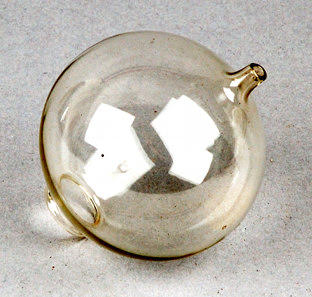
\includegraphics[width=1\linewidth]{2}
		\caption{\small\textit{\color{timhieukhoahoc}Hình $1$. Một thiết bị cộng hưởng Helmholtz.}}
		\vspace*{-10pt}
	\end{figure}
	Phương pháp của Fourier giúp Helmholtz đưa ra ý tưởng rằng các âm thanh phức tạp có thể được đơn giản hóa thành tổng của các sóng âm đơn giản hơn với các tần số khác nhau. Để tiến hành nghiên cứu vấn đề này, ông đã chế tạo các dụng cụ thí nghiệm được gọi là thiết bị cộng hưởng Helmholtz. Mỗi một thiết bị cộng hưởng Helmholtz gồm một quả cầu kim loại hoặc thủy tinh có lỗ hở ở một đầu. Đầu còn lại có một núm nhỏ để người sử dụng có thể gắn vào tai.
	\vskip 0.1cm
	Cơ chế hoạt động của thiết bị cộng hưởng này có thể được giải thích theo một mô hình tương tự với dao động của con lắc lò xo dựa trên tính đàn hồi của không khí. Khi một khối không khí đi vào hình cầu, nó sẽ đóng vai trò của vật dao động còn lượng không khí có sẵn ở trong thiết bị sẽ bị nén lại. Tương tự như lò xo bị nén, lượng khí bị nén lại này sẽ đẩy khối khi ban đầu ra ngoài xa hơn so với trước, đồng thời giãn nở ra. Do đó, không khí ở trong một vật chứa hình cầu có thể dao động tương tự như một con lắc lò xo.
	\vskip 0.2cm
	\PIbox{Bản thân các dụng cụ âm nhạc đều là các thiết bị cộng hưởng để khuyếch đại âm thanh: ống của các loại kèn, sáo, hộp đàn của các loại đàn dây, thân của các loại trống. 
		\begin{figure}[H]
			\centering
			\vspace*{-5pt}
			\captionsetup{labelformat= empty, justification=centering}
			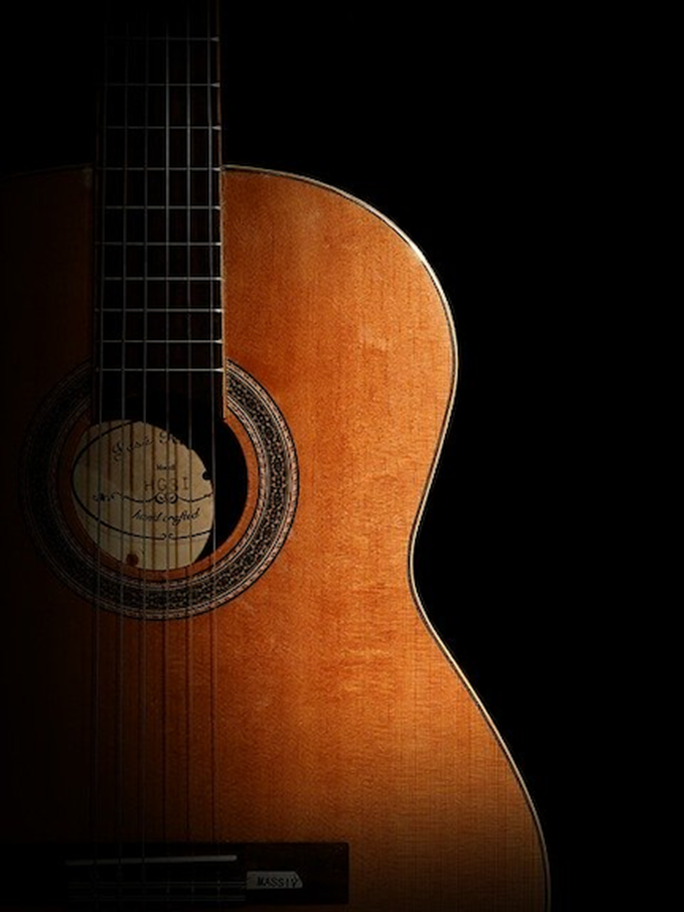
\includegraphics[width=1\linewidth]{3}
			%		\caption{\small\textit{\color{timhieukhoahoc}Hình $1$. Một thiết bị cộng hưởng Helmholtz.}}
%			\vspace*{-10pt}
	\end{figure}}
	\vskip 0.2cm
	Tùy theo kích thước hình cầu và độ rộng của lỗ, mỗi một thiết bị cộng hưởng Helmholtz có một tần số dao động tự nhiên riêng biệt. Khi sử dụng núm của thiết bị để nghe bằng cách cắm vào tai, người dùng chỉ nghe thấy các thành phần của âm thanh có tần số giống với tần số dao động tự nhiên của thiết bị còn các tần số khác đều bị suy giảm.
	Bản thân các dụng cụ âm nhạc đều là các thiết bị cộng hưởng để khuyếch đại âm thanh: ống của các loại kèn, sáo, hộp đàn của các loại đàn dây, thân của các loại trống. 
	\begin{figure}[H]
		\centering
		\vspace*{-5pt}
		\captionsetup{labelformat= empty, justification=centering}
		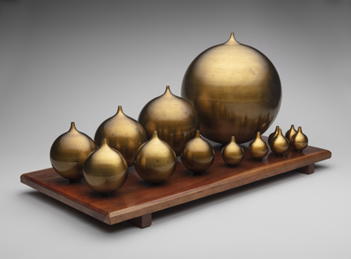
\includegraphics[width=1\linewidth]{4}
		\caption{\small\textit{\color{timhieukhoahoc}Hình $2$. Một bộ thiết bị cộng hưởng Helmholtz cho các tần số khác nhau.}}
		\vspace*{-10pt}
	\end{figure}
	Helmholtz không dừng ở việc phân tích âm thanh mà còn tiến hành các thí nghiệm tổng hợp âm thanh. Ông sử dụng các âm thoa được kích hoạt cho dao động bằng nam châm điện. Các âm thoa cấu tạo khác nhau sẽ có các tần số cơ bản khác nhau. Âm thanh của chúng sẽ được khuyếch đại bằng thiết bị cộng hưởng Helmholtz. Thông qua các thí nghiệm phân tích cũng như tổng hợp âm thanh, Helmholtz đã xác định được rằng âm thanh của các dụng cụ âm nhạc cũng như các nguyên âm trong giọng nói của con người là sự tổng hợp của những âm thanh với tần số khác nhau và ta cũng có thể tạo những âm thanh tương tự bằng cách tổng hợp các sóng âm với tần số tương ứng. Ví dụ với nguyên âm ``a”, thanh quản sẽ khuyếch đại các tần số gần với $800$ Hz, $1600$ Hz và $2400$ Hz. Với những nguyên âm khác, các cơ của cổ họng và miệng sẽ thay đổi hình dạng của thanh quản, tạo ra một bộ các tần số cộng hưởng khác. Dựa trên các công trình của Helmholtz, Graham Bell đã nảy sinh ý tưởng về việc truyền dẫn âm thanh trên dây điện theo các tần số khác nhau và tổng hợp lại thành âm thanh ban đầu, dẫn đến sự ra đời của điện thoại cố định.
	\begin{figure}[H]
		\centering
		\vspace*{-5pt}
		\captionsetup{labelformat= empty, justification=centering}
		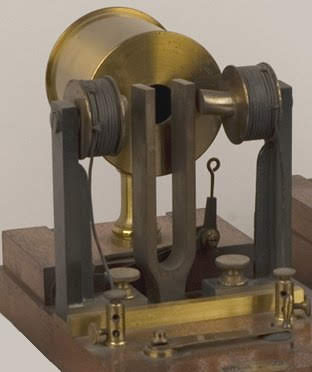
\includegraphics[width=1\linewidth]{5}
		\caption{\small\textit{\color{timhieukhoahoc}Hình $3$. Thiết bị phát sóng âm của Helmholtz.}}
		\vspace*{-10pt}
	\end{figure}
	Cũng do nghiên cứu của Helmholtz, thuật ngữ ``resonance" chính thức được sử dụng để chỉ sự dao động mãnh liệt ở một tần số đặc thù, tất nhiên lúc này vẫn chỉ giới hạn với dao động của sóng âm.
	\begin{figure}[H]
		\centering
		\vspace*{-5pt}
		\captionsetup{labelformat= empty, justification=centering}
		
\includegraphics[width=1\linewidth]{6}
		\caption{\small\textit{\color{timhieukhoahoc}Hình $4$. Chim gõ kiến sử dụng thân cây làm thiết bị cộng hưởng.}}
		\vspace*{-10pt}
	\end{figure}
	Không chỉ có con người, một số loài động vật cũng biết sử dụng hiện các vật thể trong tự nhiên làm thiết bị cộng hưởng sóng âm. Các loài chim gõ kiến sử dụng việc gõ vào thân cây để giao tiếp với nhau trong rừng nên chúng thường chọn những thân cây khô và rỗng để tăng hiệu quả cộng hưởng giúp âm thanh vang xa hơn. Trong khi đó, một số loài bướm đêm lại có các cấu trúc vảy trên cánh cộng hưởng với sóng âm mà dơi bắt mồi phát ra, khiến sóng này bị hấp thụ thay vì phản xạ lại cho dơi.
	\begin{figure}[H]
		\centering
		\vspace*{-5pt}
		\captionsetup{labelformat= empty, justification=centering}
		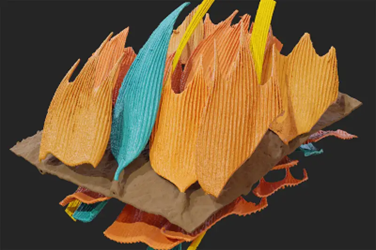
\includegraphics[width=1\linewidth]{7}
		\caption{\small\textit{\color{timhieukhoahoc}Hình $5$. Một số loài bướm đêm có cấu tạo vảy đặc thù cộng hưởng với sóng âm phát ra từ dơi bắt mồi.}}
		\vspace*{-10pt}
	\end{figure}
	$\pmb{3.}$ \textbf{\color{timhieukhoahoc}Cộng hưởng điện từ}
	\vskip 0.1cm
	Ngay khi đang làm việc với hiện tượng sóng âm, Helmholtz cũng giành sự chú ý cho một loại sóng khác trong tự nhiên. Các nghiên cứu khoa học trước đó của Faraday và Weber đã cho thấy khả năng dòng điện cũng là một hiện tượng sóng. Helmholtz cho rằng, nếu toán học có thể mô tả dao động sóng âm trong một ống hình trụ thì những phương trình tương tự cũng có thể biểu diễn chuyển động của các sóng điện trường trong mạch điện kín. Nhiều nhà khoa học đương thời khác cũng có những ý tưởng giống như vậy, bao gồm Kelvin và Maxwell. Với những công trình được công bố trong giai đoạn $1861-1865$, Maxwell đã xây dựng cơ sở toán học cho lý thuyết về sóng điện từ với hệ các phương trình mô tả dao động của các sóng này.
	\vskip 0.1cm
	Trước đó, trong công bố năm $1853$, Kelvin đã chỉ ra sự tăng vọt cường độ dòng điện trong mạch $LC$ (gồm cuộn cảm có độ tự cảm $L$ và tụ điện có điện dung $C$) khi tần số dòng xoay chiều là $\omega =\sqrt{LC}$. Phải đến năm $1885$, nhà vật lý Anton Oberbeck mới sử dụng thuật ngữ cộng hưởng mượn từ lĩnh vực sóng âm để miêu tả hiện tượng này và chỉ ra sự tương đồng về mặt phương trình của hai loại dao động, sóng âm và sóng điện từ. 
	\vskip 0.1cm
	Năm $1886$, Heinrich Hertz phát hiện rằng mạch LC phát ra sóng điện từ trong không gian mà không cần dây dẫn, cung cấp bằng chứng quan trọng khẳng định dự đoán của Maxwell. Đồng thời, thí nghiệm này cũng khẳng định sự tồn tại của cộng hưởng sóng điện từ.
	\vskip 0.1cm
	Bản thân Hertz cho rằng sóng điện từ cũng như đặc tính cộng hưởng của nó không có ứng dụng trong đời sống. Tuy nhiên thực tế lại hoàn toàn ngược lại. Dựa trên công trình của Hertz và một số nhà khoa học khác, Guglielmo Marconi đã chế tạo hệ thống thu phát sóng radio cho phép truyền tín hiệu không dây trong thực tế đồng thời thương mại hóa công nghệ này. Để tránh xung đột từ các nguồn khác nhau, cả thiết bị phát và thiết bị thu được điều chỉnh về cùng một tần số cộng hưởng. Ngày nay việc thu phát sóng không dây đã trở nên quá quen thuộc trong đời sống, từ phát thanh, truyền hình không dây cho đến điện thoại di động, Internet wifi hay các thiết bị bluetooth. Trong các công nghệ này, các mạch cộng hưởng vẫn luôn đóng vai trò thiết yếu khi thu phát tín hiệu.
		\begin{figure}[H]
		\centering
		\vspace*{-5pt}
		\captionsetup{labelformat= empty, justification=centering}
		
\includegraphics[width=1\linewidth]{8}
		\caption{\small\textit{\color{timhieukhoahoc}Hình $6$. Marconi và thiết bị thu phát sóng không dây do ông chế tạo.}}
		\vspace*{-5pt}
	\end{figure}
	\PIbox{Một dạng cộng hưởng khác ở cấp độ vi mô hơn là cộng hưởng từ hạt nhân. Khi ta kích thích một hạt nhân được đặt trong một từ trường mạnh, hạt nhân này có thể phát ra bức xạ với tần số nhất định do sự chuyển trạng thái của spin trong hạt nhân. Sự cộng hưởng này được sử dụng để quan sát bên trong các mẫu vật cũng như chụp cắt lớp cộng hưởng từ (MRI) trong y học.
	\begin{figure}[H]
		\centering
		\vspace*{-5pt}
		\captionsetup{labelformat= empty, justification=centering}
		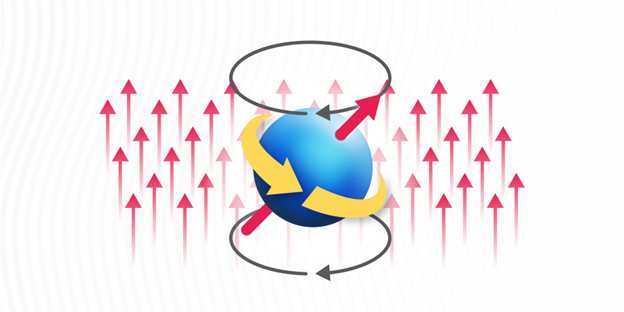
\includegraphics[width=1\linewidth]{9}
		\vspace*{-10pt}
	\end{figure}}
	\vskip 0.2cm
	$\pmb{4.}$ \textbf{\color{timhieukhoahoc}Cộng hưởng và cơ học ứng dụng}
	\vskip 0.1cm
	Quá trình để lý thuyết cộng hưởng được chấp nhận trong cơ học ứng dụng kéo dài suốt từ thế kỷ $19$ đến đầu thế kỷ $20$. Năm $1831$, cầu treo Broughton ở Anh bị sập do binh lính tiến hành hành quân theo nhịp bước trên cầu. Một sự kiện tương tự cũng xảy ra ở Angers, Pháp năm $1850$. Năm $1855$, Redtenbacher, một giáo sư cơ học ở Karlsruhe, ghi nhận rằng khi vận tốc của động cơ tàu hỏa tăng dần, sẽ có một giá trị của vận tốc khiến dao động của thân tàu bị tăng đột biến, có thể gây ra tai nạn. Tuy nhiên, khi vận tốc vượt qua giá trị này thì biên độ dao động cũng giảm theo. Ông cũng chỉ ra sự liên hệ giữa quan sát này và hiện tượng cộng hưởng nhưng các phân tích của Redtenbacher bị giới học thuật lúc đó phủ nhận.
	\vskip 0.1cm
	Đến đầu thế kỷ $20$, cộng hưởng trong các thiết bị cơ học mới được quan tâm trở lại. Kỹ sư đóng tàu Hermann Frahm chú ý đến sự cộng hưởng cơ học của các tàu đi biển trên đại dương với dao động sóng biển có thể làm cho tàu bị dao động mạnh và lật. Để giảm bớt ảnh hưởng có hại của việc này, ông thiết kế hệ thống bể chứa nước ở hai bên thành tàu có pha dao động ngược với pha dao động của tàu. Do phát minh này, ông được Arrhenius đưa vào danh sách đề cử giải Nobel vật lý năm $1913$. Ngoài thiết bị cho tàu biển, Frahm còn có nhiều sáng chế khác để giảm ảnh hưởng của cộng hưởng trong các hệ thống cơ học khác nhau.
	\begin{figure}[H]
		\centering
		\vspace*{-5pt}
		\captionsetup{labelformat= empty, justification=centering}
		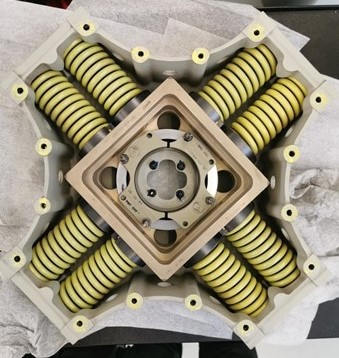
\includegraphics[width=1\linewidth]{10}
		\caption{\small\textit{\color{timhieukhoahoc}Hình $7$. Một thiết bị giảm dao động cho cánh quạt trực thăng phát triển từ bằng sáng chế của Frahm.}}
		\vspace*{-10pt}
	\end{figure}
	Đồng thời, các nhà toán học như Felix Klein và Arnold Sommerfeld cũng công bố và biên soạn các tài liệu khoa học có liên quan đến cộng hưởng trong cơ học. Dần dần, vấn đề cộng hưởng cũng trở thành một nội dung thiết yếu trong chương trình học của các kỹ sư. Trong khi các công trình lớn của thế kỷ $19$, như cầu Brooklyn hay tháp Eiffel chỉ được thiết kế dựa trên các công thức tĩnh học thì trong thế kỷ $20$, việc thiết kế và đánh giá an toàn của các công trình cũng như thiết bị cơ học đều tính đến quá trình vận hành và chuyển động, đặc biệt là tác động của các dao động tự nhiên như gió hay động đất đến các công trình. Có thể thấy, tuy được biết đến từ sớm thông qua các nhận định về con lắc đơn của Galileo, cộng hưởng cơ học lại mất thời gian rất dài, tới vài thế kỷ, để trở nên phổ biến trong các tài liệu khoa học và kỹ thuật cũng như trong ứng dụng thực tiễn. 
	\vskip 0.1cm
	\PIbox{Một ví dụ khá thú vị gần đây về cộng hưởng cơ học là việc một bản nhạc năm $2022$ của ca sĩ Janet Jackson có tần số gây ra cộng hưởng với một số ổ đĩa cứng laptop. Nếu một người mở bản nhạc này trên laptop hoặc bản nhạc được phát trên một thiết bị gần đó, dao động cộng hưởng cơ học có thể phá hủy các đĩa trong ổ cứng của laptop. Các ổ cứng bị ảnh hưởng đều có tốc độ quay $5400$ vòng/phút và được sản xuất khoảng những năm $2005$! Cũng may là các ổ cứng cơ học sản xuất gần đây không bị ảnh hưởng bởi tần số của bài hát này.
	\vskip 0.1cm
	\begin{figure}[H]
		\centering
		\vspace*{-5pt}
		\captionsetup{labelformat= empty, justification=centering}
		
\includegraphics[width=1\linewidth]{11}
		\vspace*{-10pt}
	\end{figure}
	}
	\vskip 0.1cm
	$\pmb{6.}$ \textbf{\color{timhieukhoahoc}Kết luận}
	\vskip 0.1cm
	Cộng hưởng là một hiện tượng khá thú vị xảy ra trong nhiều lĩnh vực khác nhau. Việc giảng dạy về hiện tượng này sẽ trở nên thú vị hơn nếu chúng ta đưa vào các nội dung liên quan đến lịch sử khoa học cũng như mô hình toán học của nó.
	\vskip 0.1cm
	\textbf{\color{timhieukhoahoc}Phụ lục: Mô hình toán học của hiện tượng cộng hưởng}
	\vskip 0.1cm
	\setlength{\abovedisplayskip}{6pt}
	\setlength{\belowdisplayskip}{6pt}
	Xét một con lắc lò xo với vật khối lượng $m$ và lò xo độ cứng $k$. Lực đàn hồi phụ thuộc vào ly độ $x$ của vật so với vị trí cân bằng:
	\begin{align*}
		F=-kx,
	\end{align*}
	(dấu $-$ xuất hiện do lực ngược chiều với sự biến dạng của lò xo).
	\vskip 0.1cm
	Theo định luật $2$ Newton:
	\begin{align*}
		mx''=ma=-kx,
	\end{align*}
	hay:
	\begin{align*}
		x''+\omega_0^2 x=0,		\tag{$1$}
	\end{align*}
	với $\omega_0 = \sqrt{\dfrac{k}{m}}$ và $x''$ là đạo hàm cấp $2$ của $x$ theo thời gian $t$.
	\vskip 0.1cm 
	Đây cũng là phương trình dao động của con lắc lò xo trong sách giáo khoa vật lí $12$.
	\vskip 0.1cm
	Từ dạng của phương trình này, ta thấy rằng $x$ là một hàm số mà khi lấy đạo hàm sẽ được một hàm số là tích của hàm số ban đầu với một hằng số. Một hàm số thỏa mãn dạng này là $f(t) = e^{\lambda t}$. Thay $f(x)$ vào phương trình dao động và rút gọn ta được:
	\begin{align*}
		\lambda^2 + \omega_0^2 = 0,
	\end{align*}
	hay 
	\begin{align*}
		\lambda = \pm i \omega_0.
	\end{align*}
	Do các giá trị $\lambda$ tìm được là số phức, ta sử dụng công thức Euler:
	\begin{align*}
		e^{ix} = \cos x + i \sin x.
	\end{align*}
	Khi đó, ta được $x_1 = \cos\omega_0t + i\sin\omega_0t$ và $x_2 = \cos \omega_0t - i\sin \omega_0t$.
	\vskip 0.1cm
	Do phương trình ($1$) của ta là phương trình vi phân tuyến tính (cấp hai) nên các tổ hợp tuyến tính của hai hàm số trên cũng là nghiệm của ($1$), cho nên $\cos\omega_0t = \dfrac{1}{2}(x_1 + x_2)$ và $\sin \omega_0t = \dfrac{1}{2i}(x_1-x_2)$ cũng là nghiệm của ($1$).
	\vskip 0.1cm
	Người ta chứng minh được rằng nếu biết $n$ nghiệm độc lập của phương trình vi phân tuyến tính cấp $n$ thì nghiệm tổng quát sẽ là tổ hợp tuyến tính của $n$ nghiệm này. Vì vậy, ($1$) có nghiệm tổng quát:
	\begin{align*}
		x(t) = A \cos \omega_0t + B \sin \omega_0t,
	\end{align*}
	với $A$ và $B$ là các hằng số phụ thuộc vào giá trị ban đầu của $x$ (ly độ) và $x'$ (vận tốc) tại thời điểm $t=0$. Nghiệm này cũng có thể thu gọn thành dạng:
	\begin{align*}
		x(t) = C \cos(\omega_0t - \phi),
	\end{align*}
	và do đó ta thu được một dao động điều hòa.
	\vskip 0.1cm
	Trong trường hợp dao động còn chịu lực cản tỉ lệ với vận tốc ($F_c=-cx'$), phương trình ($1$) trở thành:
	\begin{align*}
		x'' + \dfrac{c}{m}x' + \omega_0^2x = 0, \tag{$2$}
	\end{align*}
	và phương trình của $\lambda$ có dạng:
	\begin{align*}
		\lambda^2 + \frac{c}{m} \lambda + \dfrac{k}{m} = 0. \tag{$3$}
	\end{align*}
	Trong trường hợp hai nghiệm của ($3$) là hai nghiệm thực (lực cản mạnh ứng với $c^2>4mk$), nghiệm tổng quát của ($2$) sẽ là:
	\begin{align*}
		x(t) = c_1e^{-(\alpha-\beta)t}+ c_2e^{-(\alpha + \beta)t},
	\end{align*}
	với $\alpha = \dfrac{c}{2m}, \beta = \dfrac{1}{2m}\sqrt{c^2 - 4mk}$.
	\vskip 0.1cm
	Dao động này sẽ giảm dần theo hàm mũ.
	\vskip 0.1cm
	Trong trường hợp lực cản yếu ($c^2<4mk$), ta thu được nghiệm tổng quát:
	\begin{align*}
		x(t) = Ce^{-\alpha t}\cos(\omega_*t - \phi),
	\end{align*}
	với $\omega_* = \sqrt{\dfrac{k}{m} - \dfrac{c^2}{4m^2}}$.
	\vskip 0.1cm
	Đây là một dao động có biên độ giảm dần theo thời gian.
	\begin{figure}[H]
		\centering
		\vspace*{-5pt}
		\captionsetup{labelformat= empty, justification=centering}
		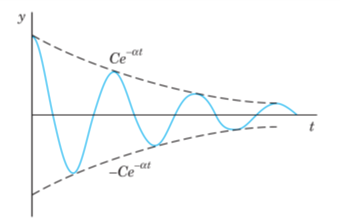
\includegraphics[width=1\linewidth]{12}
		\vspace*{-15pt}
	\end{figure}
	Trong trường hợp dao động cưỡng bức với ngoại lực cũng có tính chu kỳ, ta có phương trình:
	\begin{align*}
		mx'' + cx' + kx = F_0\cos \omega t. \tag{$4$}
	\end{align*}
	Với dạng phương trình này, nghiệm cuối cùng sẽ là tổng của nghiệm tổng quát của ($2$) và một nghiệm đặc thù thỏa mãn ($4$).
	\vskip 0.1cm
	Ta tìm một nghiệm đặc thù có dạng tương tự với vế phải:
	\begin{align*}
		x_p(t) = a \cos \omega_t + b\sin\omega_t.
	\end{align*}
	Đây còn gọi là phương pháp  hệ số bất định. Thay biểu thức của $x_p$ vào ($4$) ta được:
	\begin{align*}
		&[(k - m\omega^2)a + \omega b]\cos\omega t \\
		&+  [-\omega ca + (k- m\omega^2)b]\sin \omega t = F_0\cos \omega t.
	\end{align*}
	Cân bằng các hệ số của $\sin\omega t$ và $\cos\omega t$ ta được hệ phương trình gồm hai phương trình và hai ẩn. Khi giải hệ ta được:
	\begin{align*}
		&a = F_0 \dfrac{m(\omega_0^2 - \omega^2)}{m^2(\omega_0^2 - \omega^2)^2 + \omega^2c^2},\\
		&b = F_0 \dfrac{\omega c}{m^2(\omega_0^2 - \omega^2)^2 + \omega^2c^2}.
	\end{align*}
	Nghiệm tổng quát sẽ có dạng:
	\begin{align*}
		x(t) = x_h(t) + x_p(t),
	\end{align*}
	với $x_h$ là nghiệm tổng quát của ($2$).
	\vskip 0.1cm
	Trong trường hợp không có lực cản ($c=0$), $x_p$ có dạng:
	\begin{align*}
		x_p(t) = \dfrac{F_0}{m(\omega_0^2 - \omega^2)}\cos(\omega t).
	\end{align*}
	Khi $\omega = \omega_0$ hay tần số của ngoại lực bằng với tần số dao động tự nhiên của con lắc, sử dụng quy tắc L'Hospital để lấy giới hạn, ta có:
	\begin{align*}
		\mathop {\lim }\limits_{\omega  \to {\omega _0}} {x_p} &= \frac{{{F_0}}}{m}\mathop {\lim }\limits_{\omega  \to {\omega _0}} \frac{{\frac{d}{{d\omega }}\cos (\omega t)}}{{\frac{d}{{d\omega }}\cos (\omega _0^2 - {\omega ^2})}} \\
		&= \frac{{{F_0}}}{m}\mathop {\lim }\limits_{\omega  \to {\omega _0}} \left( {\frac{{ - t\sin \omega t}}{{ - 2\omega }}} \right)\\
		& = \frac{{{F_0}}}{{2m{\omega _0}}}t\sin \omega t.
	\end{align*}
	Đây cũng là công thức mà Euler tìm ra. Khi đó, biên độ của dao động cưỡng bức sẽ tăng tuyến tính theo thời gian và cộng hưởng xảy ra.
	\vskip 0.1cm
	Trong trường hợp có lực cản, biên độ của $x_p$ sẽ là $C^*=\sqrt{a^2 + b^2}$. Lấy đạo hàm theo $\omega$ và tìm cực trị, sẽ thấy $C^*$ có giá trị lớn nhất khi $\omega = \omega_0^2 - \dfrac{c^2}{2m^2}$. Trong trường hợp này, tần số xảy ra cộng hưởng không trùng nhưng rất gần với tần số dao động tự do của con lắc lò xo khi lực cản yếu.
	\begin{figure}[H]
		\centering
		\vspace*{-5pt}
		\captionsetup{labelformat= empty, justification=centering}
		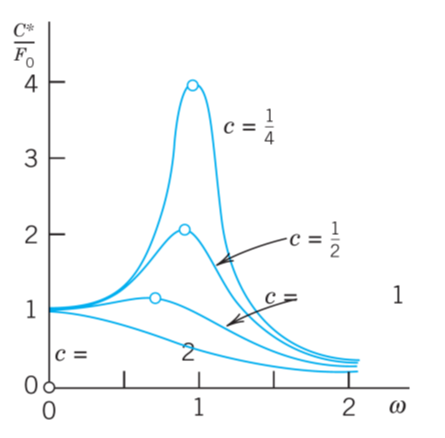
\includegraphics[width=1\linewidth]{13}
		\vspace*{-15pt}
	\end{figure}
	\textbf{\color{timhieukhoahoc}Tài liệu tham khảo}
	\vskip 0.1cm
	[$1$] Buchanan, M. ($2019$). Going into resonance. \textit{Nature Physics}, $15(3)$, $203-203$. \url{https://doi.org/10.1038/s41567-019-0458-z}
	\vskip 0.1cm
	[$2$] Eckert, M. ($2013$). \textit{Arnold Sommerfeld}. Springer Science \& Business Media.
	\vskip 0.1cm
	[$3$] Patton, L. ($2018$). Hermann von Helmholtz (Stanford Encyclopedia of Philosophy). Retrieved from Stanford.edu website: \url{https://plato.stanford.edu/entries/hermann-helmholtz/}
	\vskip 0.1cm
	[$4$] Zill, D. G. ($2018$). \textit{Advanced engineering mathematics}. Burlington: Jones \& Bartlett Learning. C.
\end{multicols}


